\section{Bevölkerungsdichten der Landkreise und Regierungsbezirke}
In \autoref{fig:distribution_incidences_counties} sind die Summe der 7-Tages Inzidenzen der einzelnen Landkreise dargestellt. Auf der linken Seite befindet sich die Verteilung und auf der rechten Seite die räumliche Anordnung.

\begin{figure}[H]
    \centering
    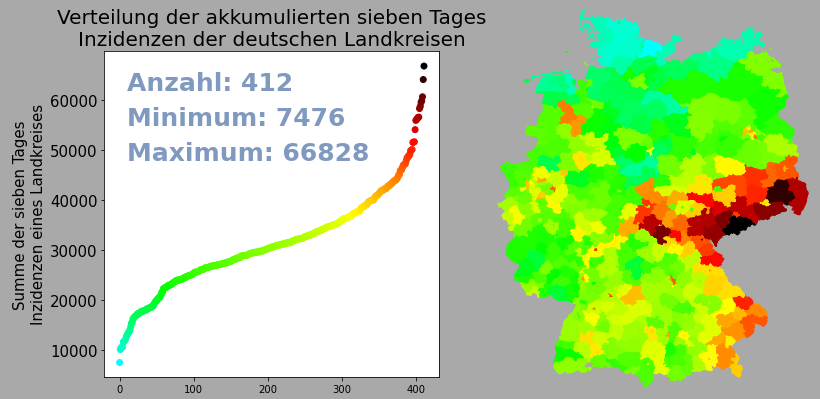
\includegraphics[width = 0.95\textwidth]{figures/Ergebnisse/accumulation_incidences_counties.png}
    \caption{Verteilung der Summe der 7-Tages Inzidenzen unter den deutschen Landkreisen.}
    \label{fig:distribution_incidences_counties}
\end{figure}

In \autoref{fig:distribution_incidences_districts} sind die Bevölkerungsdichten der einzelnen Regierungsbezirke dargestellt. Auf der linken Seite befindet sich die Verteilung und auf der rechten Seite die räumliche Anordnung.

\begin{figure}[H]
    \centering
    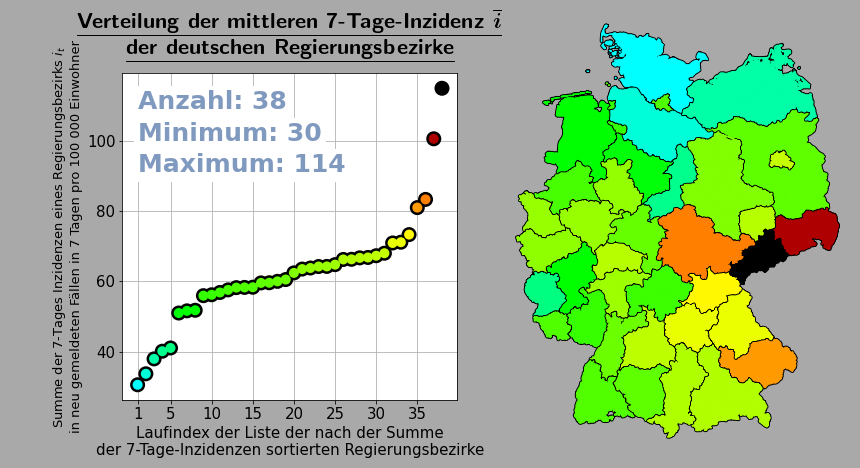
\includegraphics[width = 0.95\textwidth]{figures/Ergebnisse/accumulation_incidences_districts.png}
    \caption{Verteilung der Summe der 7-Tages Inzidenzen unter den deutschen Regierungsbezirken.}
    \label{fig:distribution_incidences_districts}
\end{figure}